\documentclass[conference]{IEEEtran}
\IEEEoverridecommandlockouts
% The preceding line is only needed to identify funding in the first footnote. If that is unneeded, please comment it out.
\usepackage{cite}
\usepackage{amsmath,amssymb,amsfonts}
\usepackage{algorithmic}
\usepackage{graphicx}
\usepackage{textcomp}
\usepackage{xcolor}
\def\BibTeX{{\rm B\kern-.05em{\sc i\kern-.025em b}\kern-.08em
T\kern-.1667em\lower.7ex\hbox{E}\kern-.125emX}}
\begin{document}

\title{CSE 6603 - Data Management in the Cloud \\ Project Report \\ Improving efficiency of Microservices Autoscaling and Scheduling with Kernel Tracing}

\author{
    \IEEEauthorblockN{Samidhya Sarker}
    \IEEEauthorblockA{Roll: \textit{1018052049} \\ \textit{CSE, BUET}}
\and
    \IEEEauthorblockN{Md. Habibur Rahman}
    \IEEEauthorblockA{Roll: \textit{0422052014} \\ \textit{CSE, BUET}}
\and
    \IEEEauthorblockN{Dr. Muhammad Abdullah Adnan}
    \IEEEauthorblockA{Professor \\ \textit{CSE, BUET}}
}

\maketitle

\begin{abstract}
Designing distributed cloud applications that are decoupled into a bunch of small components (i.e. microservices) has been made easy with microservices architecture. One of the challenges in deploying microservices is finding the optimal amount of resources (i.e. size) and the number of instances (i.e. replicas) for each microservice so that you maintain good performance and don't waste resources or underutilize them. 
\end{abstract}

\begin{IEEEkeywords}
    cloud, linux, lttng, microservice, container
\end{IEEEkeywords}

\section{Introduction}
\subsection{Cloud Computing}
Hundreds of small, fine-grained components (referred to as "microservices") work together to serve end-user requests in a distributed environment under the microservices architecture, a recent and growingly popular paradigm for developing interactive and user-facing services [1, 4, 10, 16, 35]. There are various advantages to splitting up an application into smaller microservices. It enables several development teams to independently operate on disparate microservices that may be technologically dissimilar [61]. Additionally, because each microservice may grow and operate independently based on its own state and incoming workload, the program as a whole performs better and is more reliable [63]. A microservices architecture may also make it easier to debug performance and accuracy problems \cite{b54}


\subsection{Microservices}

Microservice architecture is an architectural pattern that arranges an application as a collection of loosely-coupled, fine-grained services, communicating through lightweight protocols. It allows teams to develop and deploy their services independently of others.

Interfaces need to be designed carefully and treated as a public API.

One technique that is used is having multiple interfaces on the same service, or multiple versions of the same service, so as to not disrupt existing users of the code. \cite{b3}

Decomposing an application into different smaller services can provide several benefits, such as modularity, scalability, integration of heterogeneous and legacy systems, and continuous integration, continuous delivery and deployment.

\begin{figure}
    \begin{center}
        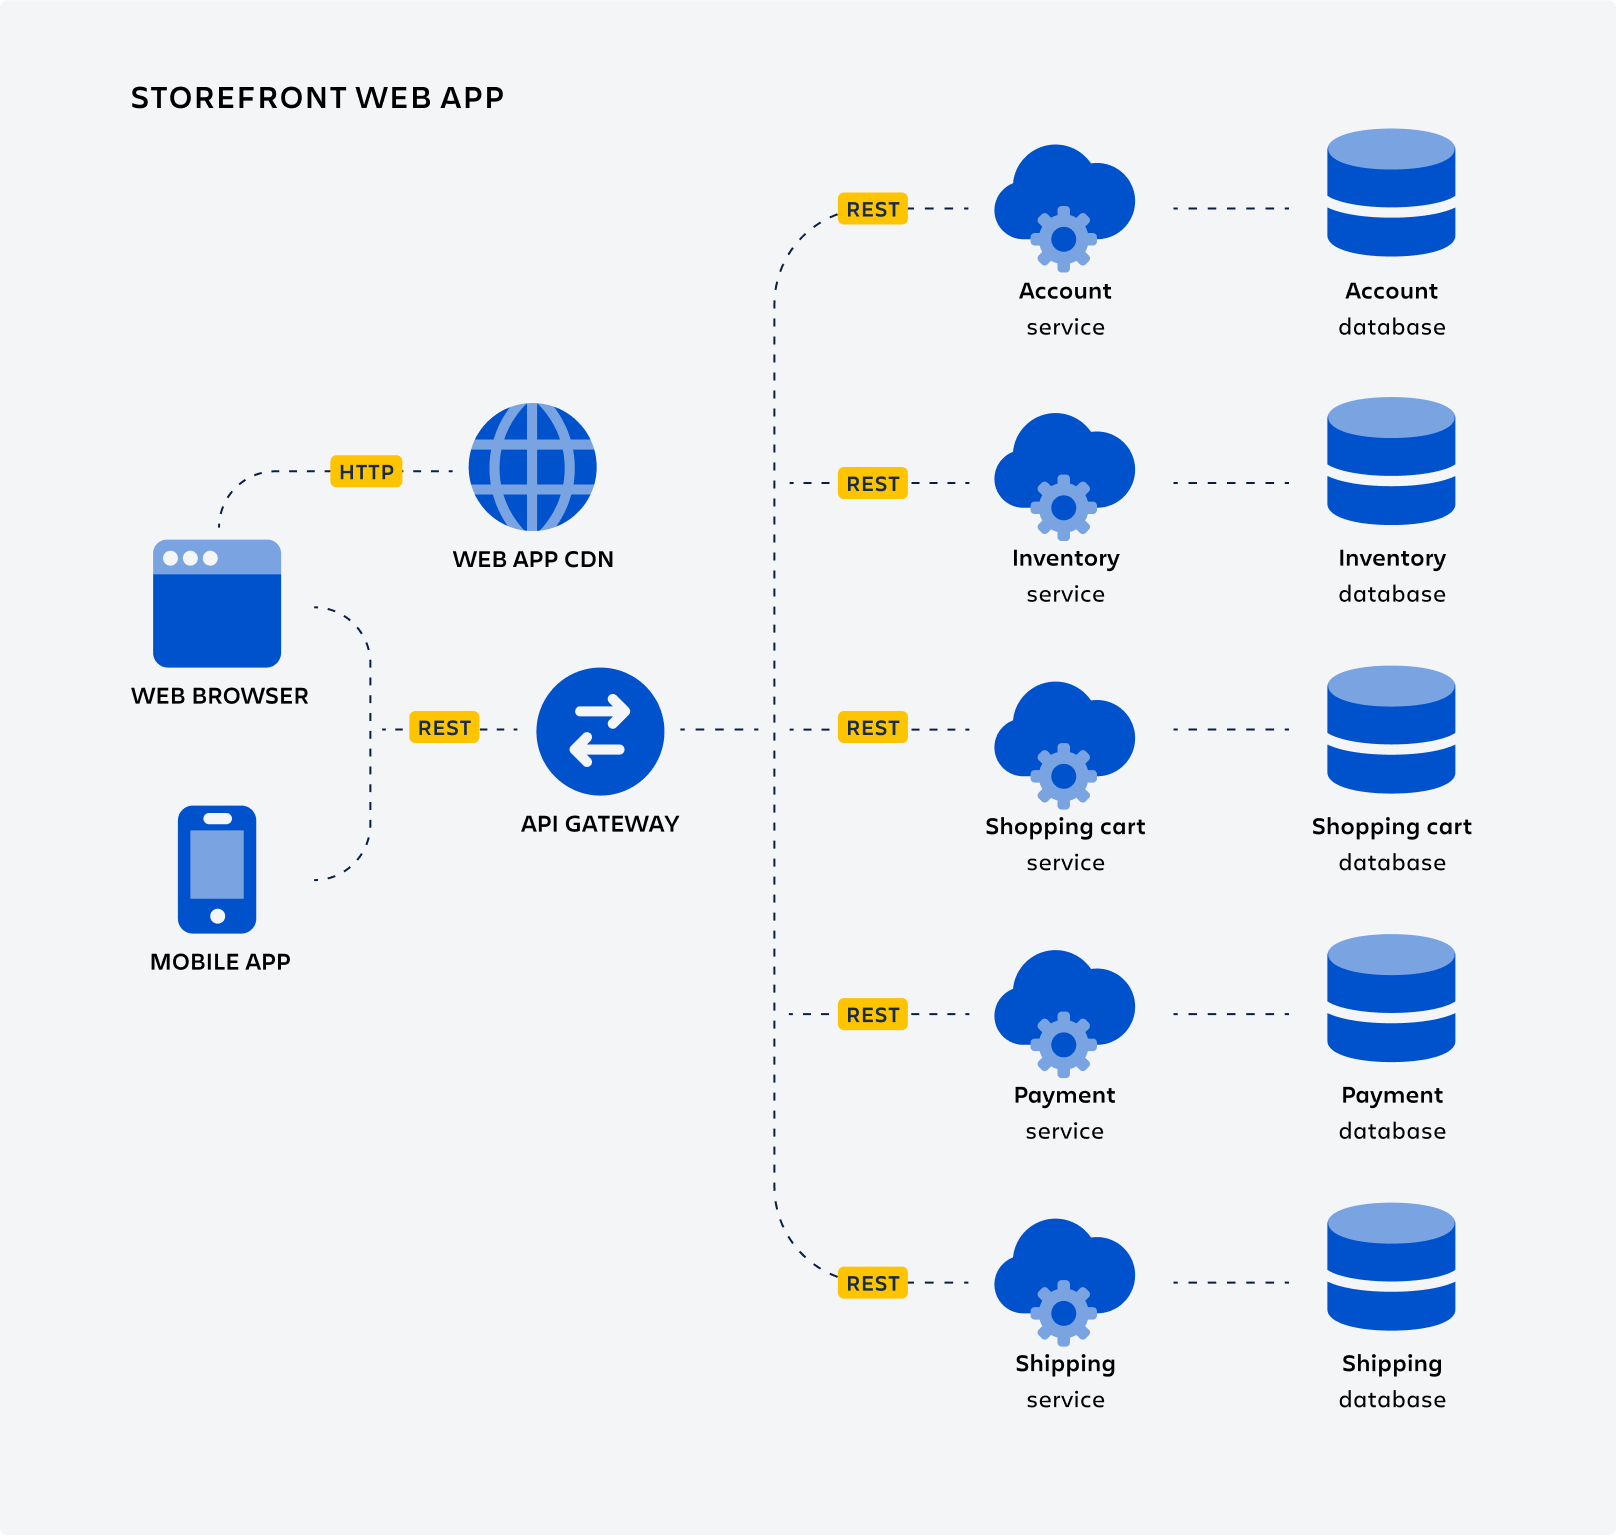
\includegraphics[width=0.3\textwidth]{figures/microservice.png}
    \end{center}
    \caption{Microservices architecture}
    \label{fig:2}
\end{figure}


\subsection{Kubernetes}

Kubernetes is a container-based platform that manages applications based on CPU, memory, or custom metrics. It is loosely coupled and extensible to meet different workloads.

Kubernetes is a platform for scheduling and running containers on clusters of physical or virtual machines (VMs). It helps you fully implement and rely on a container-based infrastructure in production environments. Developers can also create cloud-native apps with Kubernetes as a runtime platform by using Kubernetes patterns.

\subsubsection{Autoscaling}
The standard basis for autoscaling and scheduling in Kubernetes is resource utilization metrics.
\begin{figure}
    \begin{center}
        
\includegraphics[width=0.3\textwidth]{figures/kubernetes.png}
    \end{center}
    \caption{Kubernetes}
    \label{fig:Kubernetes}
\end{figure}

\subsection{Tracing}

Tracing is the specialized use of logging to record information about a program’s flow of execution.
Trace logs are used by programmers for debugging purposes, and by system administrators to diagnose common problems with software.

Several tools currently being used for tracing inside linux kernelspace. 

\subsubsection{ebpf}

eBPF is an advanced technology to run applications inside the kernel, but it is also heavier than purpose-built tracer like lttng

\subsection{Distributed Tracing}
                                                                                                                     Tracing the execution of a computer program is not a new concept, but modern architectures such as microservices have fundamentally broken the classic methods of profiling, debugging, and monitoring. Distributed tracing stands ready to fix these issues, but can be hard.
                                                                                                                     In a distributed system a daemon process running on a system can be measured in several dimensions, including the amount of memory mapped to the process. We can view open file handles, calculate CPU utilization, and do all sorts of things, but we can't trace the application.

\section{Motivation}
Microservices autoscaling in the cloud is directly linked with the cost of running the operation.

Many types of public and private Cloud systems require their users to declare how many instances their workload will need during execution, and the resources needed for each. Such limits make cloud computing possible, by enabling the Cloud infrastructure to provide adequate performance isolation. But limits are (mostly) a nuisance to the user.

\section{Related Work}

Some work has been done for enhancing the efficiency by utilizing ML and kernel tracing.

\section{Autopilot: workload autoscaling at google.\cite{b5}}

Google uses Autopilot to configure resources automatically, adjusting both the number of concurrent tasks in a job (horizontal scaling) and the CPU/memory limits for individual tasks (vertical scaling). Autopilot reduces slack by 23\% and the number of jobs severely impacted by OOMs by a factor of 10. Despite its advantages, ensuring that Autopilot was widely adopted took significant effort, including making potential recommendations easily visible to customers who had yet to opt in, automatically migrating certain categories of jobs, and adding support for custom recommenders.

\section{Firm}
This paper presents FIRM, an intelligent fine-grained resource management framework that uses online telemetry data and machine-learning methods to predictably share resources across microservices to drive up overall utilization. FIRM reduces service level objectives (SLOs) violations by up to 16 while reducing overall requested CPU limit by up to 62\%.
\subsection{Showar\cite{b4}}
SHOWAR shows a 22\% improvement with eBPF tracing.

\section{Experimentation}

\subsection{System Setup}

\begin{figure}
    \begin{center}
        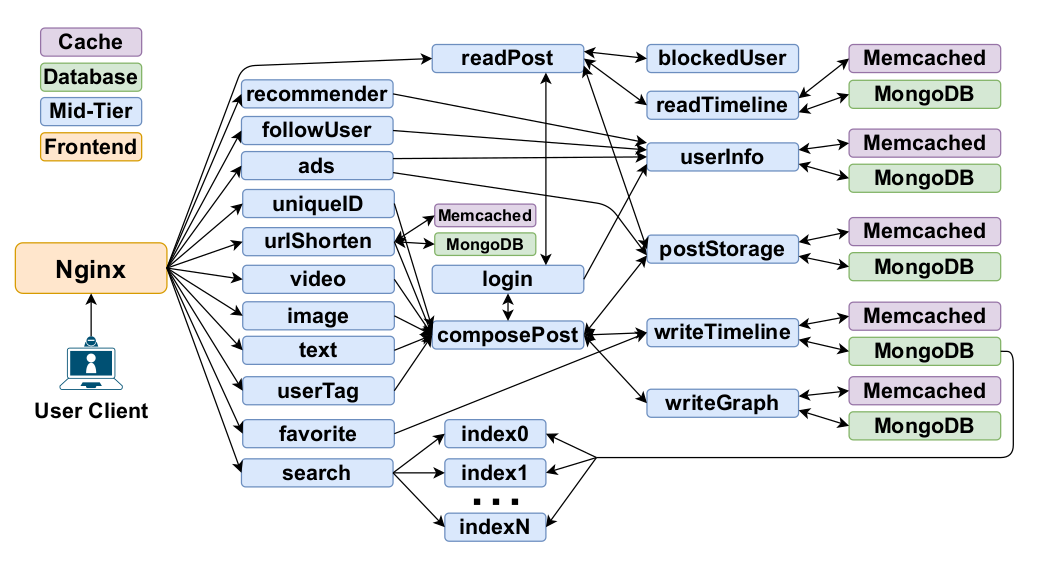
\includegraphics[width=0.4\textwidth]{figures/social-network.png}
    \end{center}
    \caption{DeathStarbench\cite{b2} Social Network application using microservices architecture}
    \label{fig:social-network}
\end{figure}


\begin{thebibliography}{00}
    \bibitem{b54} Austin Parker, Daniel Spoonhower, Jonathan Mace, Ben Sigelman, and Rebecca Isaacs. 2020. Distributed tracing in practice: Instrumenting, analyzing, and debugging microservices. O’Reilly Media.
    \bibitem{b2} Yu Gan, Yanqi Zhang, Dailun Cheng, Ankitha Shetty, Priyal Rathi, Nayan Katarki, Ariana Bruno, Justin Hu, Brian Ritchken, Brendon Jackson, et al. 2019. An open-source benchmark suite for microservices and their hardware-software implications for cloud \& edge systems. In Proceedings of the Twenty-Fourth International Conference on Archi- tectural Support for Programming Languages and Operating Systems. 3–18.
    \bibitem{b3} \sloppy Martin Fowler. "Microservices". http://martinfowler.com/articles/\\microservices.html
    \bibitem{b4} Baarzi, Ataollah Fatahi, and George Kesidis. "Showar: Right-sizing and efficient scheduling of microservices." Proceedings of the ACM Symposium on Cloud Computing. 2021.
    \bibitem{b5} Rzadca, Krzysztof, et al. "Autopilot: workload autoscaling at google." Proceedings of the Fifteenth European Conference on Computer Systems. 2020.
    \bibitem{b6} 
\end{thebibliography}
\end{document}
